\documentclass[12pt,a4paper]{article}
\usepackage{amsmath,amscd,amsbsy,amssymb,latexsym,url,bm,amsthm}
\usepackage{epsfig,graphicx,subfigure}
\usepackage{enumitem,balance}
\usepackage{wrapfig}
\usepackage{mathrsfs,euscript}
\usepackage[usenames]{xcolor}
\usepackage{hyperref}
\usepackage[vlined,ruled,linesnumbered]{algorithm2e}
\usepackage{float}
\hypersetup{colorlinks=true,linkcolor=black}

\newtheorem{theorem}{Theorem}
\newtheorem{lemma}[theorem]{Lemma}
\newtheorem{proposition}[theorem]{Proposition}
\newtheorem{corollary}[theorem]{Corollary}
\newtheorem{exercise}{Exercise}
\newtheorem*{solution}{Solution}
\newtheorem{definition}{Definition}
\theoremstyle{definition}

\renewcommand{\thefootnote}{\fnsymbol{footnote}}

\newcommand{\postscript}[2]
 {\setlength{\epsfxsize}{#2\hsize}
  \centerline{\epsfbox{#1}}}

\renewcommand{\baselinestretch}{1.0}

\setlength{\oddsidemargin}{-0.365in}
\setlength{\evensidemargin}{-0.365in}
\setlength{\topmargin}{-0.3in}
\setlength{\headheight}{0in}
\setlength{\headsep}{0in}
\setlength{\textheight}{10.1in}
\setlength{\textwidth}{7in}
\makeatletter \renewenvironment{proof}[1][Proof] {\par\pushQED{\qed}\normalfont\topsep6\p@\@plus6\p@\relax\trivlist\item[\hskip\labelsep\bfseries#1\@addpunct{.}]\ignorespaces}{\popQED\endtrivlist\@endpefalse} \makeatother
\makeatletter
\renewenvironment{solution}[1][Solution] {\par\pushQED{\qed}\normalfont\topsep6\p@\@plus6\p@\relax\trivlist\item[\hskip\labelsep\bfseries#1\@addpunct{.}]\ignorespaces}{\popQED\endtrivlist\@endpefalse} \makeatother

\begin{document}

\noindent

%========================================================================
\noindent\framebox[\linewidth]{\shortstack[c]{
\Large{\textbf{Lab04-Matroid}}\vspace{1mm}\\
CS214-Algorithm and Complexity, Xiaofeng Gao, Spring 2021.}}
\begin{center}
\footnotesize{\color{red}$*$ If there is any problem, please contact TA Haolin Zhou.}

% Please write down your name, student id and email.
\footnotesize{\color{blue}$*$ Name: Yanjie Ze  \quad Student ID:519021910706 \quad Email:zeyanjie@sjtu.edu.cn}
\end{center}
%第一题
\begin{enumerate}
\item \textit{Property of Matroid.} 
\begin{enumerate}
	\item
	Consider an arbitrary undirected graph $ G=(V,E) $. Let us define $ M_{G}=(S,C) $ where $ S=E $ and $ C=\left\{I \subseteq E \mid\left(V, E \backslash I\right) \text { is connected}\right\} $. Prove that $ M_{G} $ is a \textbf{matroid}.\par
	    \begin{proof}
	    ~\\
{\color{blue}Hereditary}: Suppose $A\subset B, B\in C$.

$B$ satisfies that $(V, E\backslash B)$ is connected.

$A\subset B$, so $(V, E\backslash A)$ is connected too.

Therefore, $A\in C$.
~\\

{\color{blue}Exchange Property}: Denote two subsets $A, B\in C$, $|A| < |B|$. Assume edge $x\in B, x\notin A$. Then:$E\backslash (A\cup \{x\}) = E\backslash A) \cup E\backslash \{x\}$

	   \end{proof}
	\item
	Given a set $A$ containing $n$ real numbers, and you are allowed to choose $k$ numbers from $A$. The bigger the sum of the chosen numbers is, the better. What is your algorithm to choose? Prove its correctness using \textbf{matroid}.\par
	\textbf{Remark:} Denote $\mathbf{C}$ be the collection of all subsets of $A$ that contains no more than $k$ elements. Try to prove $(A,\mathbf{C})$ is a matroid.\par
	   \begin{solution}
	   ~\\
	   The greedy algorithm is optimal in this problem, shown in Alg.~\ref{alg1}.
	   
	      \begin{algorithm}[H]
   \caption{Greedy Choice}\label{alg1}
		Sort all numbers in $A$ into ordering $x_1\geq x_2\geq ...\geq x_n$\;
		$S\leftarrow \emptyset$\;
		
		\For{$i=1$ to $k$}{
		$S\cup \{x_i\}$\;	
		}
		\Return $S$\;	
	\end{algorithm}
	    \end{solution}
\begin{proof}
~\\
Denote $\mathbf{C}$ be the collection of all subsets of $A$ that contains no more than $k$ elements.We try to prove  $(A,\mathbf{C})$ is a matroid.

{\color{blue}Hereditary}: Denote $A\subset B\in \mathbf{C}$. $B$ contains no more than $k$ elements. So $A$ also contains no more than $k$ elements.

{\color{blue}Exchange Property}: Denote $A, B\in C$, $|A|<|B|$. Assume $x\in B, x\notin A$. 

Since $|A|<|B|\leq k$, $|A\cup \{x\}|\leq k$. Therefore, $A\cup \{x\} \in C$.

Thus, $(A,\mathbf{C})$ is a matroid.\par

~\\
\textbf{Lemma}: If $(S, \mathbf{C}, c)$ is a weighted matroid, then Greedy-MAX algorithm performs the optimal solution.\par

In this problem, cost function $c(x_i)=x_i$, meaning the larger the number, the more weights it has. And we have proved that $(A, \mathbf{C})$ is a matroid. Therefore, Alg.~\ref{alg1} is optimal.

\end{proof}
\end{enumerate}

%第二题
\item \textit{Unit-time Task Scheduling Problem.} Consider the instance of the \textbf{Unit-time Task Scheduling Problem} given in class. 
    \begin{enumerate}
        \item Each penalty $\omega_{i}$ is replaced by $80-\omega_{i}$. The modified instance is given in Tab.~\ref{tab:1}. Give the final schedule and the optimal penalty of the new instance using Greedy-MAX.
		\begin{table}[H]
			\setlength{\abovecaptionskip}{0.cm}
			\setlength{\belowcaptionskip}{0.5cm}
			\centering
			\caption{Task}
			\label{tab:1}			
			\begin{tabular}{|c|ccccccc|}
				\hline
				$ a_{i} $&1&2&3&4&5&6&7\\
				\hline
				$ d_{i} $&4&2&4&3&1&4&6\\
                \hline
                $ \omega_{i} $&10&20&30&40&50&60&70\\
				\hline
			\end{tabular}
		\end{table}
	        \begin{solution}
	        ~\\
	       Let S be a set of unit-time tasks with deadlines and \textbf{C} the set of all independent tasks of S. Then $(S, \mathbf{C}) $ is matroid and Alg.~\ref{alg2} Greedy-MAX is optimal.
	       
	        \begin{algorithm}[H]
   \caption{Greedy-MAX}\label{alg2}
		Sort all penalties  into ordering $w_1\geq w_2\geq ...\geq w_n$\;
		$S\leftarrow \emptyset$\;
		
		\For{$i=1$ to $n$}{
		\If{$S\cup \{w_i\} \in \mathbf{C}$\;}{$S \leftarrow S\cup \{x_i\}$\;}	
		}
		\Return $S$\;	
	\end{algorithm}
	
For the tasks in table.~\ref{tab:1}, we can start to select from $i=7$. Greedy-MAX selects $a_7, a_6, a_5,a_4,a_3$, then rejects $a_2, a_1$.

The final schedule is $<a_5, a_4, a_6,a_3,a_7>$, which is shown in Fig.~\ref{task}.

The optimal penalty is $w_2 + w_1 = 30$.


\begin{figure}[htbp]
    \centering
    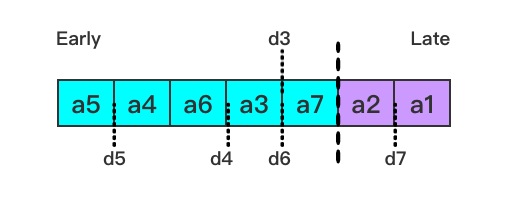
\includegraphics[width=0.6\textwidth]{explain1.png}
    \caption{Task Scheduling}\label{task}
\end{figure}


	    \end{solution}
        \item Show how to determine in time $O(|A|)$ whether or not a given set $A$ of tasks is independent. (\textbf{Hint}: You can use the lemma of equivalence given in class)
 	       \begin{solution}
	       ~\\
	      \textbf{Lemma:} For any set of tasks A, the two statements are equivalent.
	      \begin{enumerate}
	      \item The set A is independent.
	      \item For $t=0,1,2,...,n$, $N_t(A)\leq t$.
	   \end{enumerate}
	   
	  Based on the lemma, we are able to design an algorithm to utilize the property of $N_t(A)$, shown in Alg.~\ref{alg3}.
		
		\begin{algorithm}[H]
   \caption{Independent Judging}\label{alg3}
		\textbf{Input:} task set $A$ \;
		Define array $a[|A|]$\;
		Define array $N[|A|]$\;
		Define $sum:=0$\;
		\For{$i=1$ to $|A|$}{
			$a[d_i]++$\;
		}
		\For{$i=1$ to $|A|$}{
		$sum += a[i]$\;
		$N[i] := sum$\;
		\If{$N[i]>i$}{
		\Return False
		}
		}
		\Return True		
	\end{algorithm}


\textbf{Explanation of the algorithm}: 

First, we define an array $a$ to record the deadlines. It has the size of $|A|$, because the maximum of the deadline is not more than $|A|$. $a[i]$ means the number of tasks with the deadline $i$. 

Second, we define an array $N$ to function as $N_t(A)$ in the lemma. $N[i]$ means the number of tasks in $A$ whose deadline is $i$ or earlier. This array is actually not necessary and we can only use $sum$, but this array helps understand the algorithm and does not increase the upper bound of the time complexity.

Third, we will explain the loops. The first loop is to count the appearances of deadlines. The second loop is proposed to calculate the cumulative deadlines. 
~\\

\textbf{Time complexity}: $O(|A|)$

The two loop both have a $O(|A|)$ time complexity.
~\\

\textbf{Space complexity}: $O(|A|)$

To count deadlines, we need at least one array $a$, with size equal to $|A|$. The array $N$ is not necessary as mentioned before and it does not effect the complexity. Therefore, the overall space complexity is $O(|A|)$.

            \end{solution}
    \end{enumerate}
%第三题
\item \textit{MAX-3DM.} Let $X$, $Y$, $Z$ be three sets. We say two triples $\left(x_{1}, y_{1}, z_{1}\right)$ and $\left(x_{2}, y_{2}, z_{2}\right)$ in $X \times Y \times Z$ are \textit{disjoint} if $x_{1} \neq x_{2}$, $y_{1} \neq y_{2},$ and $z_{1} \neq z_{2}$. Consider the following problem:
    
    \begin{definition}[MAX-3DM] 
        Given three disjoint sets $X$, $Y$, $Z$ and a non-negative weight function $c(\cdot)$ on all triples in $X \times Y \times Z$, \textbf{Maximum 3-Dimensional Matching} (MAX-3DM) is to find a collection $\mathcal{F}$ of disjoint triples with maximum total weight.
    \end{definition}

    \begin{enumerate}
    	\item Let $D = X \times Y \times Z$. Define independent sets for MAX-3DM.
	 \begin{solution}
	 ~\\
	    Define $\mathbf{H}=\{F\subseteq D| \forall (x_1,y_1,z_1), (x_2,y_2,z_2)\in F, they\ are\ disjoint.\}$
	    
	    {\color{blue}Hereditary}: Denote $A\subset B, B\in \mathbf{H}$. Since triples in $B$ are all disjoint, triples in $A$ are disjoint. Thus $A\in \mathbf{H}$.
	    
	    $(D, \mathbf{H})$ is an \textbf{independent system}. Each subset $F$ in $\mathbf{H}$ is \textbf{independent}.
    	    \end{solution}
	    
    	\item Write a greedy algorithm based on Greedy-MAX in the form of \emph{pseudo code}. \label{Item-Greedy}
	\begin{solution}
	~\\	
	Greedy-MAX has been mentioned in Alg.~\ref{alg2}. Greedy-MAX combined with 3DM problem is shown in Alg.~\ref{alg4}, called Greedy-MAX-3DM. The basic ideas in them are the same.
	
		\begin{algorithm}[H]
   \caption{Greedy-MAX-3DM}\label{alg4}
		Sort all weights into ordering: $c(x_1,y_1,z_1)\geq c(x_2,y_2,z_2) \geq ... \geq c(x_n,y_n,z_n)$\;
		$\mathcal{F} \leftarrow \emptyset $\;
		\For{$i=1$ to $n$}{
		\If{$\mathcal{F} \cup \{(x_i,y_i,z_i)\} \in \mathbf{H} $}
		{
			$\mathcal{F} \leftarrow \mathcal{F} \cup \{(x_i,y_i,z_i)\}$\;
		}
		}
		\Return $\mathcal{F}$\;
	\end{algorithm}

	\end{solution}
	
    	\item Give a counter-example to show that your Greedy-MAX algorithm in Q.~\ref{Item-Greedy} is not optimal.
	\begin{solution}
	~\\
	The instance setting is shown in table.~\ref{tab:2}. 
	
	\textbf{Greedy-MAX-3DM}: $\mathcal{F} = \{ (0,0,0), (3,3,3)\}, weight=5+2=7$
	
	\textbf{Optimal}: $\mathcal{F} = \{ (1,0,1), (2,2,0),(3,3,3)\}, weight=4+3+2=9$

	\begin{table}[H]
			\setlength{\abovecaptionskip}{0.cm}
			\setlength{\belowcaptionskip}{0.5cm}
			\centering
			\caption{Task}
			\label{tab:2}			
			\begin{tabular}{|c|c|c|c|}
				\hline
				$ x_i$ & $y_i$ & $z_i$ & $weight$\\
				\hline
				0&0&0&5\\
				\hline
				1&0&1&4\\
				\hline
				2&2&0&3\\
				\hline
				3&3&3&2\\
				\hline
					
			\end{tabular}
		\end{table}
	\end{solution}
    	\item Show that: $\max\limits_{F \subseteq D} \frac{v(F)}{u(F)} \leq 3$. {\color{blue}(Hint: you may need Theorem~\ref{Thm-Intersect} for this subquestion.)} 
    	    \begin{solution}
	    ~\\
	    \textbf{We construct 3 matroids and construct the independent system based on the 3 matroids.}
	    
	    Define $\mathbf{S}=\{F\subseteq D| \forall (x_1,y_1,z_1), (x_2,y_2,z_2) \in F, x_1\neq x_2 \}$
	    
	    	    Define $\mathbf{R}=\{F\subseteq D| \forall (x_1,y_1,z_1), (x_2,y_2,z_2) \in F, y_1\neq y_2 \}$
		    
		    	    Define $\mathbf{T}=\{F\subseteq D| \forall (x_1,y_1,z_1), (x_2,y_2,z_2) \in F, z_1\neq z_2 \}$
		
		We prove that    $(D, \mathbf{S})$, $(D, \mathbf{R})$, $(D, \mathbf{T})$ are all matroids.
		
	\begin{proof}
	~\\
	For $(D, \mathbf{S})$:
	
	{\color{blue}Hereditary}: Denote $A\subset B \in \mathbf{S}, |A|<|B|$. 
	
	Because: $\forall (x_1,y_1,z_1), (x_2,y_2,z_2) \in B, x_1\neq x_2 $.
	
	Thus: $\forall (x_1,y_1,z_1), (x_2,y_2,z_2) \in A, x_1\neq x_2 $.
	
	Therefore, $A\in \mathbf{S}$.
	
		{\color{blue}Exchange Property}: Denote two subsets $A, B \in \mathbf{S}, |A| < |B|$.
		
		Since $|A|<|B|$, there must exist $(x, y, z)\in B$ which satisfies $\forall (x_i,y_i,z_i) \in A, x_i \neq x$.
		
		Therefore, $A\cup \{(x,y,z)\} \in \mathbf{S}$.
		
	Finally we prove that $(D, \mathbf{S})$ is a matroid.
~\\
	
Similarly, we can use the same way to prove $(D, \mathbf{R})$, $(D, \mathbf{T})$ are all matroids.
~\\

Now we have constructed three matroids, and naturally we want to use them to construct the target independent system:

$\mathbf{S}\cap \mathbf{R} \cap \mathbf{T} = \{F\in D| \forall (x_1,y_1,z_1), (x_2,y_2,z_2) \in F, x_1\neq x_2, y_1\neq y_2, x_3\neq y_3.\} = \mathbf{H}$

From Theorem~\ref{Thm-Intersect}, we can induce that $\max\limits_{F \subseteq D} \frac{v(F)}{u(F)} \leq 3$.
	\end{proof}
			    
    	    \end{solution}
    \end{enumerate}
    \begin{theorem} \label{Thm-Intersect}
        Suppose an independent system $(E, \mathcal{I})$ is the intersection of $k$ matroids $\left(E, \mathcal{I}_{i}\right)$, $1 \leq i \leq k$; that is, $\mathcal{I}=\bigcap_{i=1}^{k} \mathcal{I}_{i}$. Then $\max\limits_{F \subseteq E} \frac{v(F)}{u(F)} \leq k$, where $v(F)$ is the maximum size of independent subset in $F$ and $u(F)$ is the minimum size of maximal independent subset in $F$.
    \end{theorem}    
\end{enumerate}

\vspace{20pt}

\textbf{Remark:} You need to include your .pdf and .tex files in your uploaded .rar or .zip file.

%========================================================================
\end{document}
